\documentclass{article}
\usepackage[utf8]{inputenc}

\usepackage{natbib}
\usepackage{graphicx}

\title{StudentLog}
\date{May 2021}

\begin{document}

\maketitle

\section{Git General Information}

GitHub generate the contributions graphs and shows how frequently the group been contributing over the project generation.

\begin{figure}[h!]
\centering
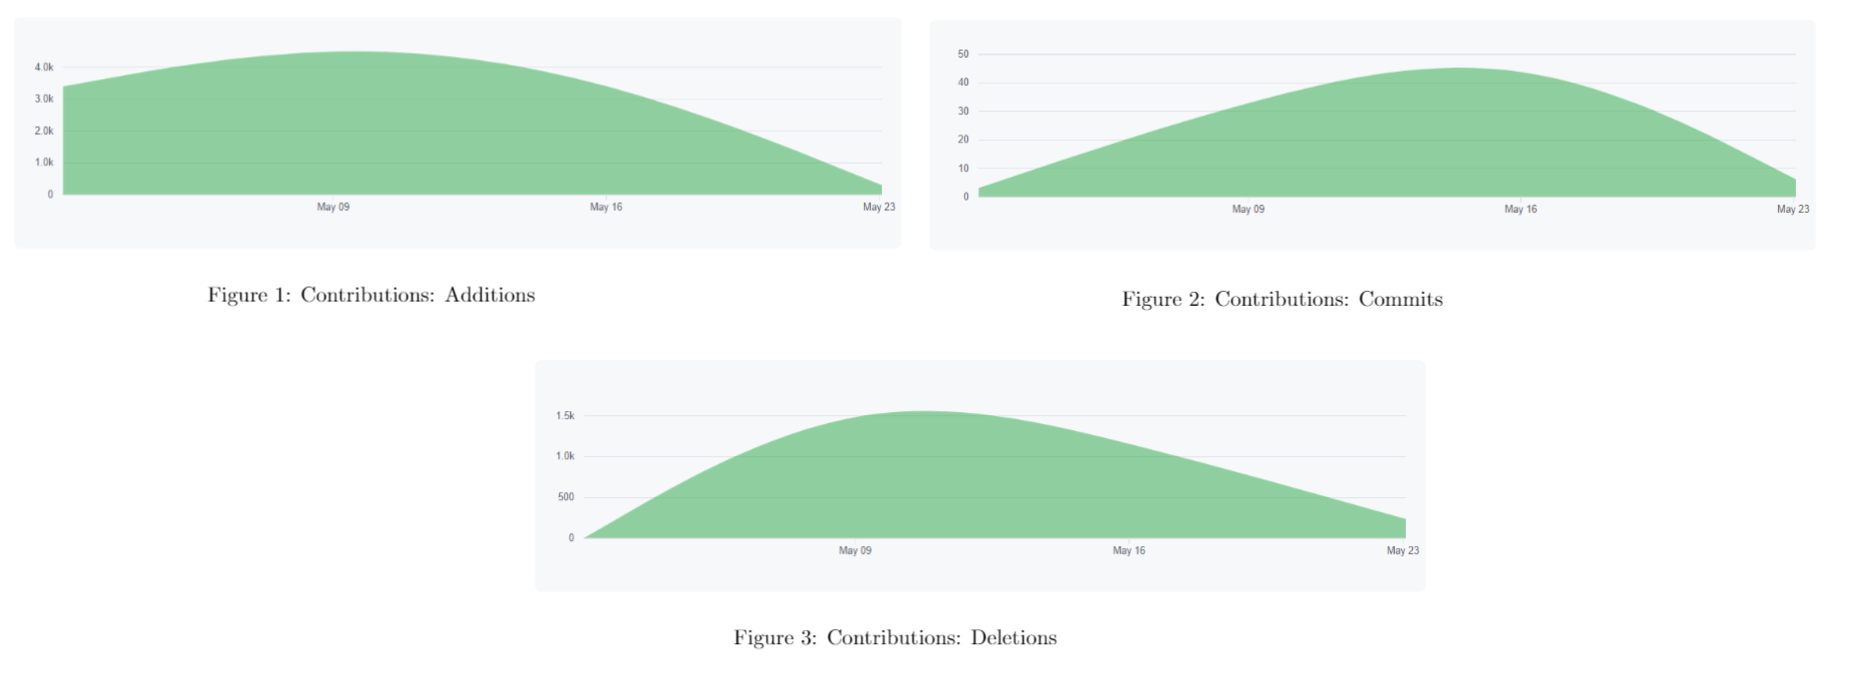
\includegraphics[width=13cm]{img/group.PNG}
\label{fig:group}
\end{figure}


The code frequency graph displays the content additions and deletions for each week in a repository's history.

\begin{figure}[h!]
\centering
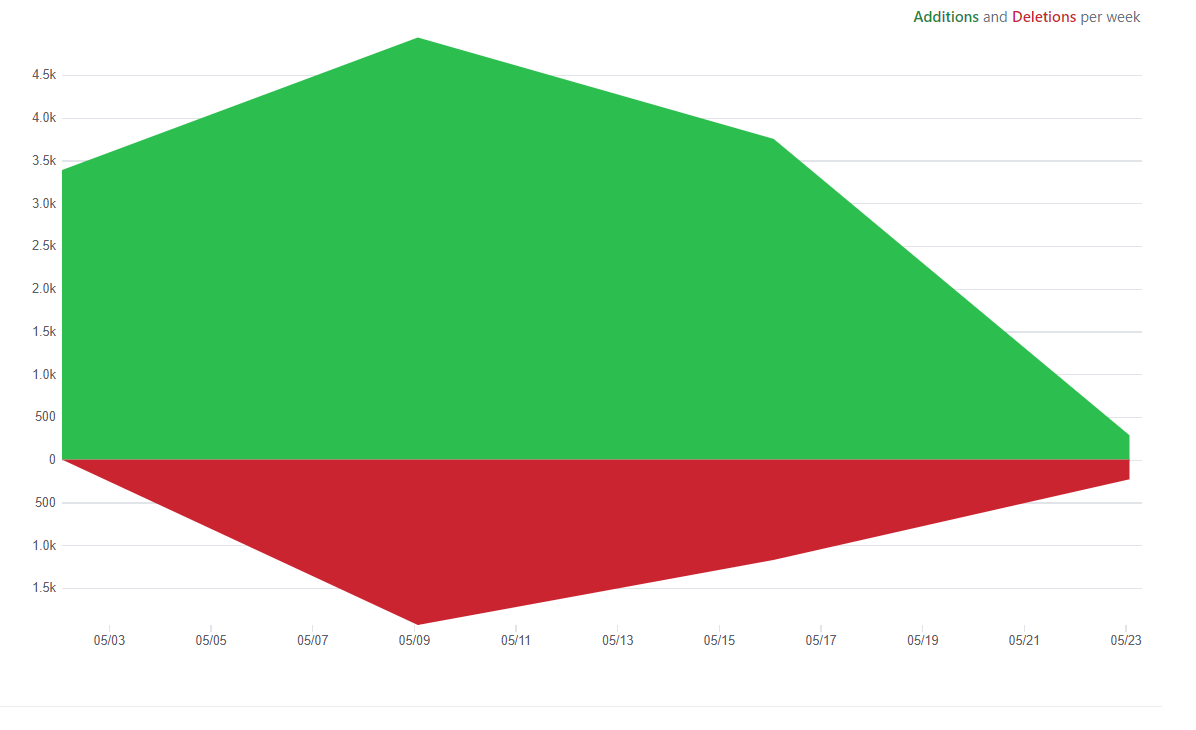
\includegraphics[width=7cm]{img/Code-frequency.PNG}
\caption{Code Frequency}
\label{fig:frequency}
\end{figure}


\section{Edoardo Cogotti}

\subsection{Git Information}

\begin{figure}[h!]
\centering
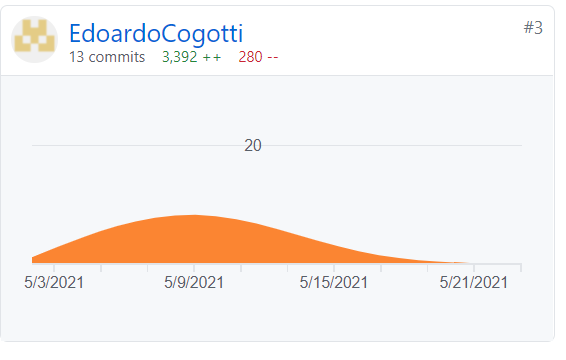
\includegraphics[width=7cm]{img/ec.PNG}
\caption{Personal Contribution. Edoardo Cogotti}
\label{fig:universe}
\end{figure}

\begin{itemize}
    \item Number of commits: \(13\)
    \item Lines of code added: \(3392\)
    \item Lines of code deleted: \(280\)
\end{itemize}

\subsection{Coding Activities}

\begin{itemize}
    \item Backend:
    \begin{itemize}
        \item DemoApplication
        \item TreasureHunt
        \item TreasureHuntStep
        \item customObject
        \item TreasureBackend
    \end{itemize}
\end{itemize}


\begin{itemize}
\item FrontEnd:
    \begin{itemize}
    \item FormMakerActivity
    \item CameraFormActivity
    \item PlaceFormActivity
    \item models/GameInfo
    \item MakerMapActivity (the skeleton, not implemented Google Maps or ML Kit API)
    \item adapters/RecycleAdapter
    \item RecapActivity (the skeleton, not implemented Google Maps)
    \item SuccessCreationActivity 
    \end{itemize}
\end{itemize}

\subsection{Diary of non Coding Activities}

\begin{itemize}
    \item Definition and implementation of database on MySql
    \item Configuration of \textbf{pom.xml} and \textbf{persistence.xml} to connect backend and database
    \item Study of java persistence and hibernate on Visual Studio Code
    \item Configuration to make static my private ip during testing on real device
    \item Study of recycleview in android studio
    \item Study of Volley
    \item Study of JsonObject
    \item Writing of the project description
\end{itemize}

\section{Marsha Gómez}

\subsection{Git Information}

\begin{figure}[h!]
\centering
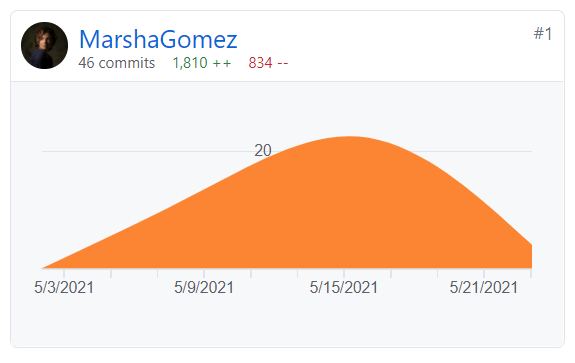
\includegraphics[width=7cm]{img/mg.PNG}
\caption{Personal Contribution. Marsha Gomez}
\label{fig:universe}
\end{figure}

\begin{itemize}
    \item Number of commits: \(46\)
    \item Lines of code added: \(1810\)
    \item Lines of code deleted: \(834\)
\end{itemize}

\subsection{Coding Activities}

\begin{itemize}
\item FrontEnd:
    \begin{itemize}
    \item models/GlobalClass
    \item GameActivity (Implementation Machine Learning Kit API)
    \item GameCameraActivity
    \item GameHangmanActivity
    \item Gradle (implementation firebase google dependencies)
    \end{itemize}
\end{itemize}

\subsection{Diary of non Coding Activities}
\begin{itemize}
    \item Study of Machine Learning Kit implementation
    \item Configuration and installation of the fire-base console for ML Kit API 
    \item Study of Mobile UX Design
    \item Participation on Design and Prototyping of the mobile application
    \item Participation on Writing of the Student Log Doc
\end{itemize}


\section{Francesco Pesciatini}

\subsection{Git Information}

\begin{figure}[h!]
\centering
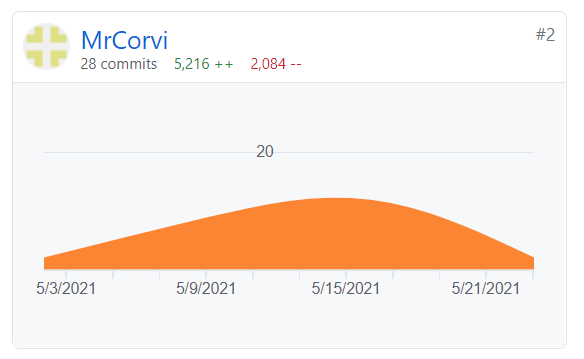
\includegraphics[width=7cm]{img/fp.PNG}
\caption{Personal Contribution. Francesco Pesciatini}
\end{figure}

\begin{itemize}
    \item Number of commits: \(28\)
    \item Lines of code added: \(5216\)
    \item Lines of code deleted: \(2084\)
\end{itemize}


\subsection{Coding Activities}

\begin{itemize}
\item FrontEnd:
    \begin{itemize}
        \item models/GlobalGame
        \item FormMakerActivity
        \item GameActivity
        \item GameStepQuestionActivity
        \item ListViewActivity
        \item MainActivity
        \item SearchGameActivity
        \item SuccessActivity
    \end{itemize}
\end{itemize}

\subsection{Diary of non Coding Activities}

\begin{itemize}
    \item Search of the best language and platform where to develop the backend
    \item Search on how to make the back end server accessible from my wifi network
    \item Study and experimentation on the use of “Intent” in android studio
    \item Research on Parcelable in android studio 
    \item Readings about how to make a UI look good in a android app
\end{itemize}

\section{Gianmarco Petrelli}

\subsection{Git Information}

\begin{figure}[h!]
\centering
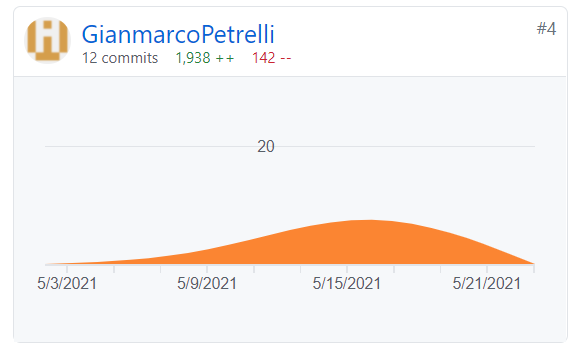
\includegraphics[width=7cm]{img/gp.PNG}
\caption{The Universe}
\label{fig:universe}
\end{figure}

\begin{itemize}
    \item Number of commits: \(12\)
    \item Lines of code added: \(1938\)
    \item Lines of code deleted: \(142\)
\end{itemize}

\subsection{Coding Activities}

Spring Boot prototipation for backend
	

\begin{itemize}
    \item FrontEnd:
    \begin{itemize}
        \item AndroidManifest
        \item MakerMapActivity (including layout)
        \item GameActivity (including layout)
        \item RecapActivity
        \item Gradle file for dependencies and Google API key management files
    \end{itemize}
    \item MySQl: update database script
	\item Building of Google map project prototype
\end{itemize}

\subsection{Diary of non Coding Activities}
\begin{itemize}
    \item Team working for project specification and moke-up
    \item Use case definition
    \item Google API prototipation
    \item Google Cloud Platform:
    \begin{itemize}
	    \item Account activation
	    \item API services activation and management
	\end{itemize}
\end{itemize}

\end{document}
